% --- FICHIER PRINCIPAL : presentation.tex ---

\documentclass{beamer}

% --- PRÉAMBULE ET PACKAGES ---
\usepackage[utf8]{inputenc}
\usepackage[T1]{fontenc} % Ajout pour une meilleure gestion des polices et accents
\usepackage[french]{babel}
\usepackage{graphicx} % Pour inclure des images et le logo
\usepackage{listings}
% --- THÈME ET APPARENCE ---
\usetheme{Madrid}             % Thème populaire avec navigation sur le côté
\usecolortheme{seahorse}           % Palette de couleurs sobre (bleu/blanc)
\setbeamertemplate{navigation symbols}{} % Cache les petits boutons de navigation

% --- INFORMATIONS DE LA PRÉSENTATION ---
% Informations mises à jour pour la cohérence avec les demandes précédentes
\title{Rapport de Projet : CryptoHack}
\author{Victor Bailleul \and Sébastien Leglise}
\institute{Université de Caen Normandie / ENSICAEN}
\date{Année 2025-2026}

% --- DÉBUT DU DOCUMENT ---
\begin{document}

    % --- SLIDE DE TITRE ---
    % La frame a été modifiée pour inclure les trois logos en pied de page.
    \begin{frame}[plain] % Ajout de l'option [plain] pour un look plus épuré sur la page de titre
        % La commande \titlepage génère la partie principale de la diapositive de titre.
        \titlepage

        % \vfill pousse tout le contenu qui suit vers le bas de la diapositive.
        \vfill

        % --- LOGOS EN PIED DE PAGE ---
        % Utilisation de l'environnement 'columns' pour aligner les trois logos côte à côte.
        % [T] aligne les colonnes par le haut, 'totalwidth' définit leur conteneur.
        \begin{columns}[T, totalwidth=\textwidth]
            % Colonne 1: Logo Unicaen
            \begin{column}{0.33\textwidth}
                \centering % Centre l'image dans la colonne
                
\includegraphics[height=2.cm]{../Main/Images/Others/logo_unicaen.png}
            \end{column}
            % Colonne 2: Logo CryptoHack
            \begin{column}{0.33\textwidth}
                \centering
                
\includegraphics[height=2cm]{../Main/Images/Others/logo_cryptohack.png}
            \end{column}
            % Colonne 3: Logo Ensicaen
            \begin{column}{0.33\textwidth}
                \centering
                
\includegraphics[height=2cm]{../Main/Images/Others/logo_ensicaen.png}
            \end{column}
        \end{columns}

        % Ajoute un petit espace vertical pour que les logos ne soient pas collés au bord.
        \vspace{0.2cm}
    \end{frame}

    % --- TABLE DES MATIÈRES ---
    % Affiche le plan de la présentation, qui est généré automatiquement.
    \begin{frame}{Plan de la présentation}
        \tableofcontents
    \end{frame}

    % --- INCLUSION DES PARTIES ---
    % Chaque partie est dans son propre fichier pour une meilleure organisation.
    % Assurez-vous que ces fichiers existent dans les répertoires correspondants.
    % --- SLIDES : Introduction ---

\section{Introduction}

\begin{frame}{Contexte du projet}

    % --- Premier bloc : Plateforme CryptoHack ---
    \begin{block}{La plateforme CryptoHack}
        \begin{itemize}
            \item Plateforme d'apprentissage dédiée à la cryptographie moderne.
            \item Approche pratique : résolution de défis à difficulté croissante.
            \item Objectif : enseigner les concepts fondamentaux et avancés.
        \end{itemize}
    \end{block}

    \vspace{0.5cm}

    % --- Deuxième bloc : Intérêt des CTF ---
    \begin{alertblock}{L'intérêt des challenges de type CTF (\textit{Capture The Flag})}
        \begin{itemize}
            \item \textbf{Principe :} \textit{Gamification} de l'apprentissage en cybersécurité.
            \item \textbf{Bénéfices :}
                \begin{itemize}
                    \item Ancrage des connaissances par la pratique.
                    \item Développement de compétences techniques (analyse, résolution de problèmes).
                \end{itemize}
        \end{itemize}
    \end{alertblock}

\end{frame}

\begin{frame}
    \frametitle{Organisation du projet}
    \framesubtitle{Planification}
    \centering
    % Remplacez 'path/to/image.png' par le chemin vers votre image.
    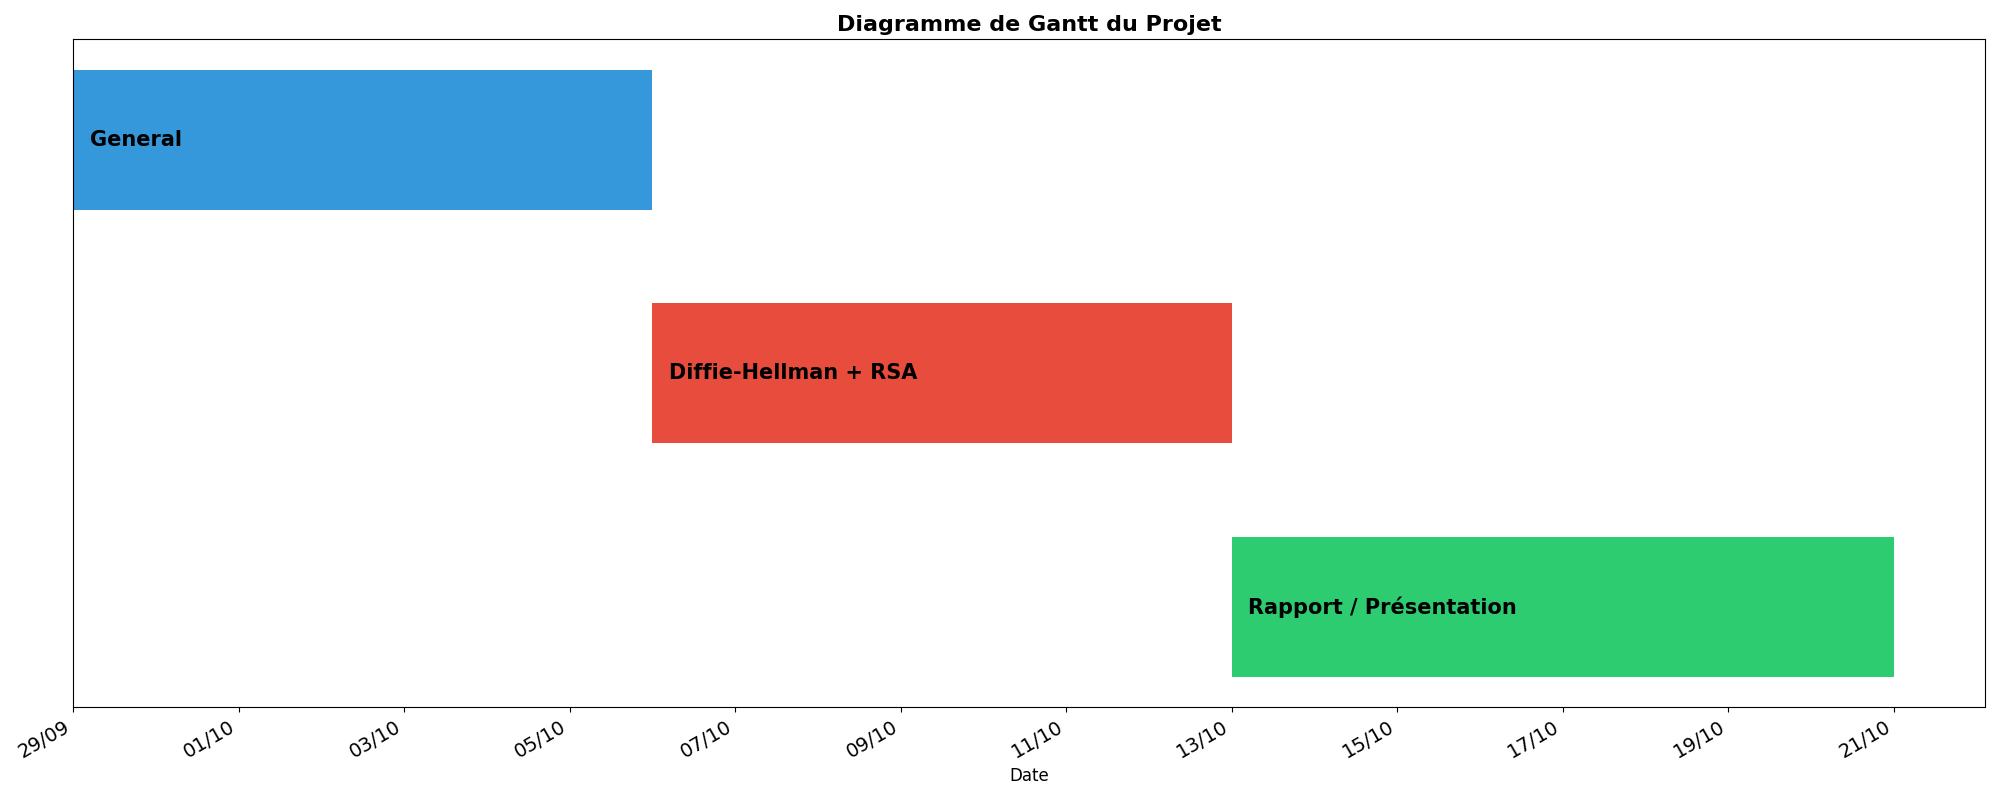
\includegraphics[width=\linewidth]{gantt.png}
\end{frame}

\begin{frame}
    \frametitle{Organisation du projet}
    \framesubtitle{Travailler en binôme}

    % --- Premier bloc : Répartition des tâches ---
    \begin{block}{Répartition des tâches individuelles}
        \centering
        \small
        \begin{tabular}{ll} 
            \textbf{} & \textit{Catégorie de challenges abordées} \\
            \textit{Victor} & General/\textbf{Encoding}, General/\textbf{XOR}, \textbf{Diffie-Hellman} \\
            \textit{Sébastien} & General/\textbf{Mathematics}, General/\textbf{Data Formats}, \textbf{RSA} \\
        \end{tabular}
    \end{block}

    \vspace{0.5cm} % Ajoute un peu d'espace entre les deux blocs

    % --- Deuxième bloc : Travail en commun ---
    \begin{alertblock}{Travail commun et collaboration}
        L'ensemble du projet a été géré via un dépôt Git partagé sur GitHub. Cette approche nous a permis de :
        \begin{itemize}
            \item \textbf{Centraliser le code} et les documents du projet.
            \item \textbf{Suivre les versions} pour éviter les conflits et les pertes de données.
            \item \textbf{Collaborer de manière asynchrone} sur les différentes parties du rapport et du code.
        \end{itemize}
    \end{alertblock}

\end{frame}
    % --- SLIDES : Challenge 1 ---

\section{Challenge Diffie-Hellman}

\begin{frame}
    \centering
    \Huge{\bfseries Challenge Diffie-Hellman}\\[1.5em]
    \huge{\textit{Man-in-the-middle}}
\end{frame}

\begin{frame}
    \frametitle{Diffie-Hellman : \textit{Man-in-the-middle | Export grade}}
    \framesubtitle{Objectifs du challenge}
    \begin{center}
        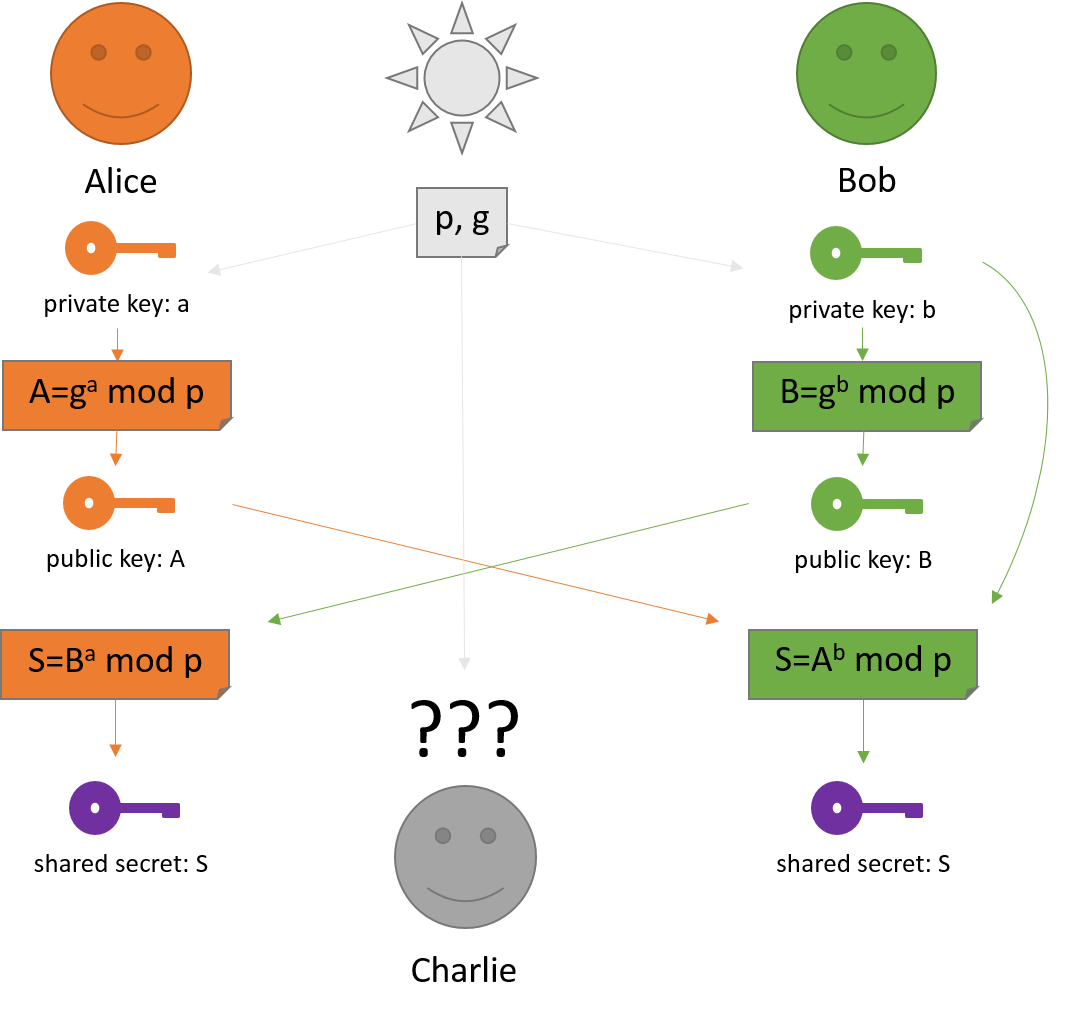
\includegraphics[width=0.65\textwidth]{diffie_key_exchange.png}
        \vspace{0.5em}
    \end{center}
\end{frame}

\begin{frame}
    \frametitle{Diffie-Hellman : \textit{Man-in-the-middle | Export grade}}
    \framesubtitle{Méthode de résolution}
    \begin{center}
        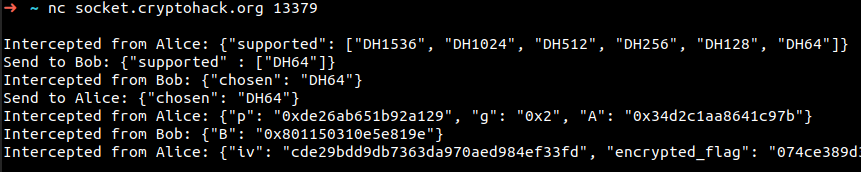
\includegraphics[width=1\textwidth,trim=0 5cm 0 0,clip]{screen_export_grade.png}
        \vspace{0.5em}
    \end{center}
\end{frame}

\begin{frame}
    \frametitle{Diffie-Hellman : \textit{Man-in-the-middle | Export grade}}
    \framesubtitle{Méthode de résolution}
    \begin{center}
        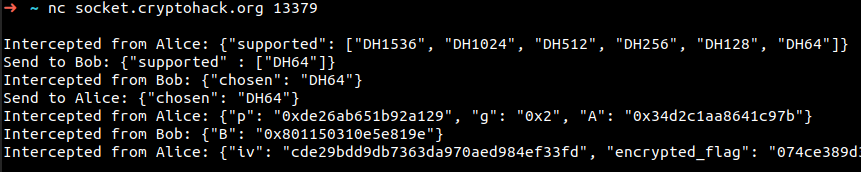
\includegraphics[width=1\textwidth,trim=0 3.5cm 0 0,clip]{screen_export_grade.png}
        \vspace{0.5em}
    \end{center}
\end{frame}

\begin{frame}
    \frametitle{Diffie-Hellman : \textit{Man-in-the-middle | Export grade}}
    \framesubtitle{Méthode de résolution}
    \begin{center}
        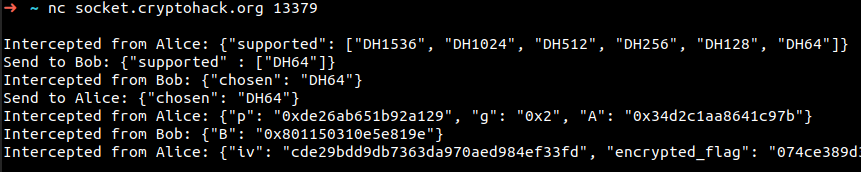
\includegraphics[width=1\textwidth,trim=0 2.2cm 0 0,clip]{screen_export_grade.png}
        \vspace{0.5em}
    \end{center}
\end{frame}

\begin{frame}
    \frametitle{Diffie-Hellman : \textit{Man-in-the-middle | Export grade}}
    \framesubtitle{Méthode de résolution}
    \begin{center}
        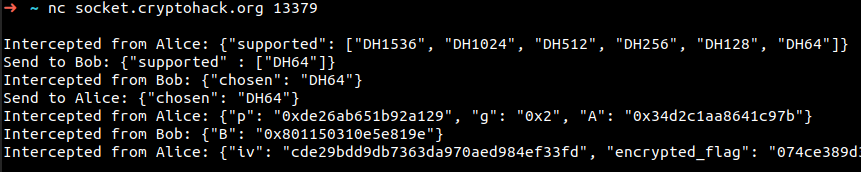
\includegraphics[width=1\textwidth]{screen_export_grade.png}
        \vspace{0.5em}
    \end{center}
\end{frame}

\begin{frame}
    \frametitle{Diffie-Hellman : \textit{Man-in-the-middle | Export grade}}
    \framesubtitle{Méthode de résolution}

    \begin{figure}
        \centering
        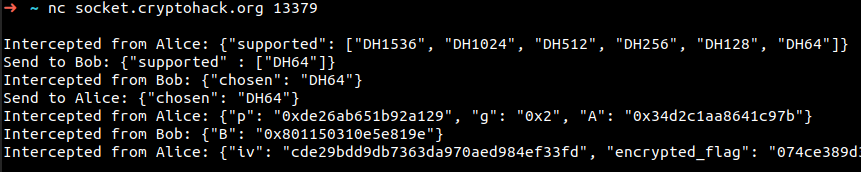
\includegraphics[width=0.9\textwidth]{screen_export_grade.png}
    \end{figure}

    \begin{block}{Étapes clés de l'attaque}
        \begin{itemize}
            \item Attaque de type \textit{Man-in-the-middle} pour manipuler la communication.
            \item Forcer Alice et Bob à utiliser un \textbf{paramètre de sécurité faible} (64 bits).
            \item La faiblesse du paramètre rend la résolution du \textbf{logarithme discret} possible, ce qui nous donne accès au secret partagé.
        \end{itemize}
    \end{block}
    
\end{frame}


\begin{frame}
    \frametitle{Diffie-Hellman : \textit{Man-in-the-middle | Export grade}}
    \framesubtitle{Résultats}

    \begin{block}{Calcul de la clé secrète partagée}
        Grâce aux paramètres faibles, nous pouvons résoudre le logarithme discret pour trouver la clé privée d'Alice ($a$) :
        $$ a = \log_g(A) \pmod{p} $$
        
        Puis, nous utilisons cette clé privée pour calculer le secret partagé ($s$) avec la clé publique de Bob ($B$) :
        $$ s = B^a \pmod{p} $$
    \end{block}
    
    \vspace{1em}
    
    Une fois le secret partagé \textit{s} obtenu, il ne reste plus qu'à dériver la clé pour obtenir le flag : 

        \begin{center}
            \Large\texttt{crypto\{d0wn6r4d35\_4r3\_d4n63r0u5\}}
        \end{center}

\end{frame}
    % --- SLIDES : Challenge 2 ---

\section{Challenge RSA}


\begin{frame}
    \centering
    \Huge{\bfseries Challenge RSA}\\[1.5em]
    \huge{\textit{Vote for Pedro}}
\end{frame}

\begin{frame}
    \frametitle{RSA : \textit{Vote for Pedro}}
    \framesubtitle{Objectifs du challenge}
\centering
{\LARGE Forger une signature RSA valide}\\
\begin{figure}
    \centering
    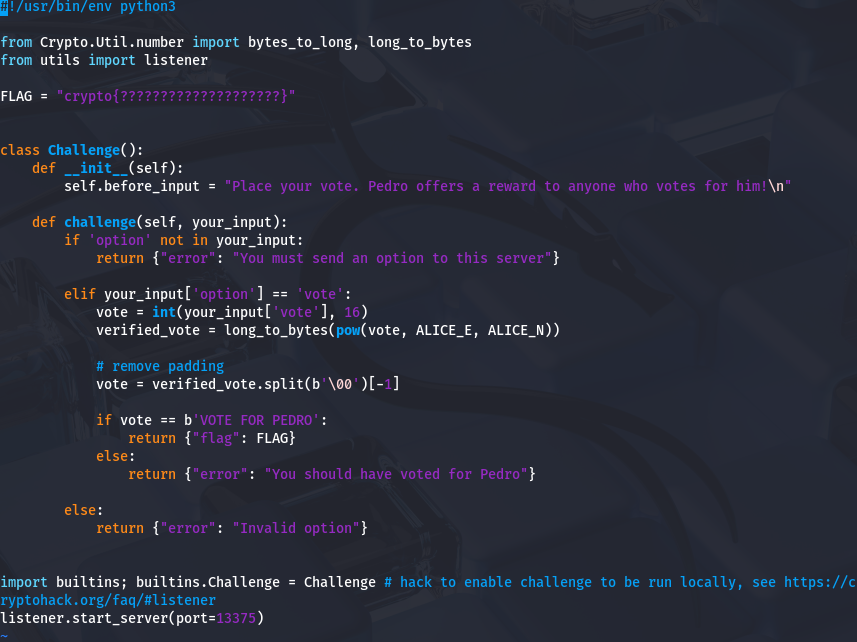
\includegraphics[width=0.5\textwidth]{scriptInitCh2.png}
\end{figure}
\vspace{0.1cm}
\begin{itemize}
    \item Voter pour Pedro sans clé privée
    \item Exploiter l'exposant faible $e = 3$
    \item Obtenir le flag
\end{itemize}
\end{frame}

\begin{frame}
    \frametitle{RSA : \textit{Vote for Pedro}}
    \framesubtitle{Méthode de résolution}
\centering
{\LARGE Attaque par racine cubique}
\vspace{0.5cm}
\begin{align*}
\text{Signature } s &= \sqrt[3]{\text{Message}} \\
s^3 &\equiv \text{Message} \pmod{N}
\end{align*}
\begin{itemize}
    \item Message court = "VOTE FOR PEDRO"
    \item Pas de padding = vulnérabilité
\end{itemize}
\end{frame}


\begin{frame}
        \frametitle{RSA : \textit{Vote for Pedro}}
    \framesubtitle{Résultats}
\centering
{\LARGE Signature forgée validée !}
\begin{figure}
    \centering
    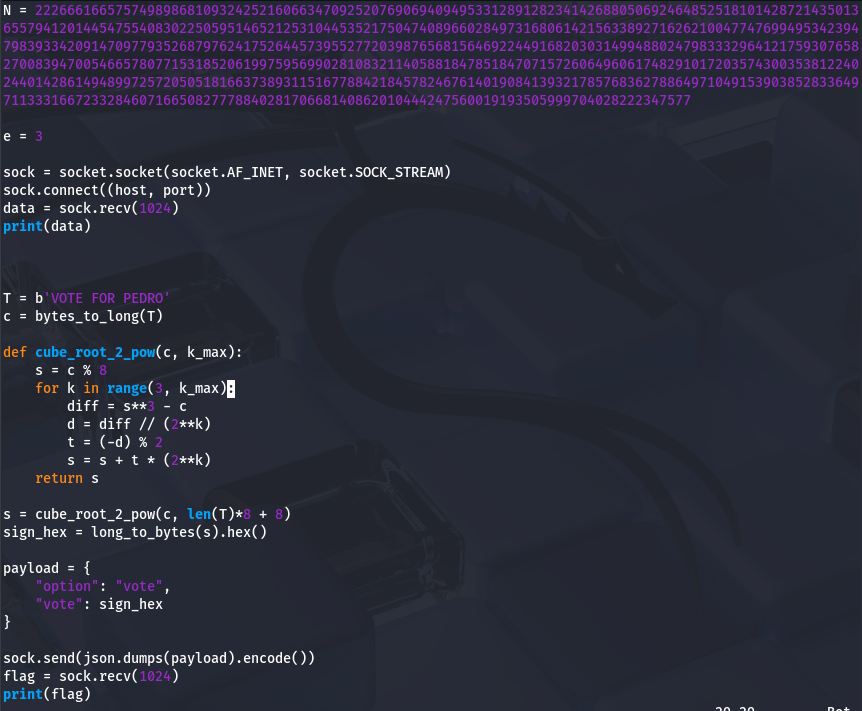
\includegraphics[width=0.5\textwidth]{scriptCh2.png}
\end{figure}
\vspace{0.1cm}
\begin{block}{Flag obtenu}
\texttt{crypto\{y0ur\_v0t3\_i5\_my\_v0t3\}}
\end{block}
\begin{itemize}
    \item Vote accepté par le serveur
\end{itemize}
\end{frame}

    % --- SLIDES : Conclusion ---

\section{Conclusion}

\begin{frame}{Bilan du projet}
    \begin{itemize}
        \item Compétences acquises.
        \item Difficultés rencontrées.
        \item Perspectives et suite possible.
    \end{itemize}
\end{frame}

\begin{frame}
    \centering
    \Huge{\bfseries Questions ?}
\end{frame}

    % --- CORRECTION D'ERREUR ---
    % L'erreur de compilation indiquait qu'un \begin{frame} dans un des fichiers inclus
    % n'avait pas de \end{frame} correspondant. On l'ajoute ici pour clore la dernière diapositive.
\end{document}

